\documentclass[11pt]{article}
\usepackage[margin=1in]{geometry}
\usepackage{booktabs}
\usepackage{graphicx}
\usepackage{hyperref}
\title{Across the Homophily Spectrum: A Controlled Study of GNNs on Node Classification}
\author{Project-2026 Team}
\date{September 2026}
\begin{document}
\maketitle
\begin{abstract}
This report studies node classification across Amazon Computers, WikiCS, and Roman-empire. The datasets move from relatively homophilic co-purchase and hyperlink graphs to a strongly heterophilic word-relationship graph. GATv2 (dynamic attention), GraphSAGE-style mean aggregation, and H2GCN (heterophily-aware design) are evaluated as GNN architectures, supplemented by MLP (feature-only) and Random (floor) baselines. All use identical task definitions and validation-selected checkpoints.
\end{abstract}
\section{Research Question}
Do GNN inductive biases transfer across graphs with different homophily, or does the best architecture depend on whether neighboring labels agree? In particular, does an architecture explicitly designed for heterophily (H2GCN) outperform general-purpose GNNs on low-homophily graphs?
\section{Datasets and Task}
We perform semi-supervised node classification. Amazon nodes are products and edges indicate co-purchase relationships. WikiCS nodes are computer-science articles and edges represent hyperlinks. Roman-empire nodes are words and edges encode the benchmark's word-relationship graph. Each dataset supplies node features and class labels with its official or deterministic split protocol.
\section{Method}
The five models represent distinct paradigms: GATv2 uses dynamic multi-head attention; GraphSAGE uses mean neighborhood aggregation in the full-batch implementation used here; H2GCN separates ego from neighbor embeddings and exploits higher-order neighborhoods for heterophilic graphs; MLP ignores graph structure entirely; and Random provides a performance floor. Learning rate and dropout are selected per model-dataset pair using validation accuracy only; the test split is not used for model selection.
\section{Results}
\begin{table}[h]
\centering
\caption{Validation-selected test results for every model-dataset pair.}
\begin{tabular}{llll}
    \toprule
Dataset & Model & Accuracy & Macro-F1 \\
\midrule
Amazon Computers & GATv2 & 0.377 & 0.086 \\
Amazon Computers & GraphSAGE & 0.375 & 0.056 \\
Amazon Computers & H2GCN & 0.375 & 0.055 \\
Amazon Computers & MLP & 0.615 & 0.264 \\
Amazon Computers & Random & 0.109 & 0.086 \\
Roman-empire & GATv2 & 0.393 & 0.285 \\
Roman-empire & GraphSAGE & 0.691 & 0.556 \\
Roman-empire & H2GCN & 0.672 & 0.484 \\
Roman-empire & MLP & 0.625 & 0.442 \\
Roman-empire & Random & 0.057 & 0.051 \\
WikiCS & GATv2 & 0.775 & 0.741 \\
WikiCS & GraphSAGE & 0.709 & 0.526 \\
WikiCS & H2GCN & 0.703 & 0.494 \\
WikiCS & MLP & 0.692 & 0.572 \\
WikiCS & Random & 0.105 & 0.091 \\
\bottomrule
\end{tabular}
\end{table}
\begin{figure}[h]
\centering
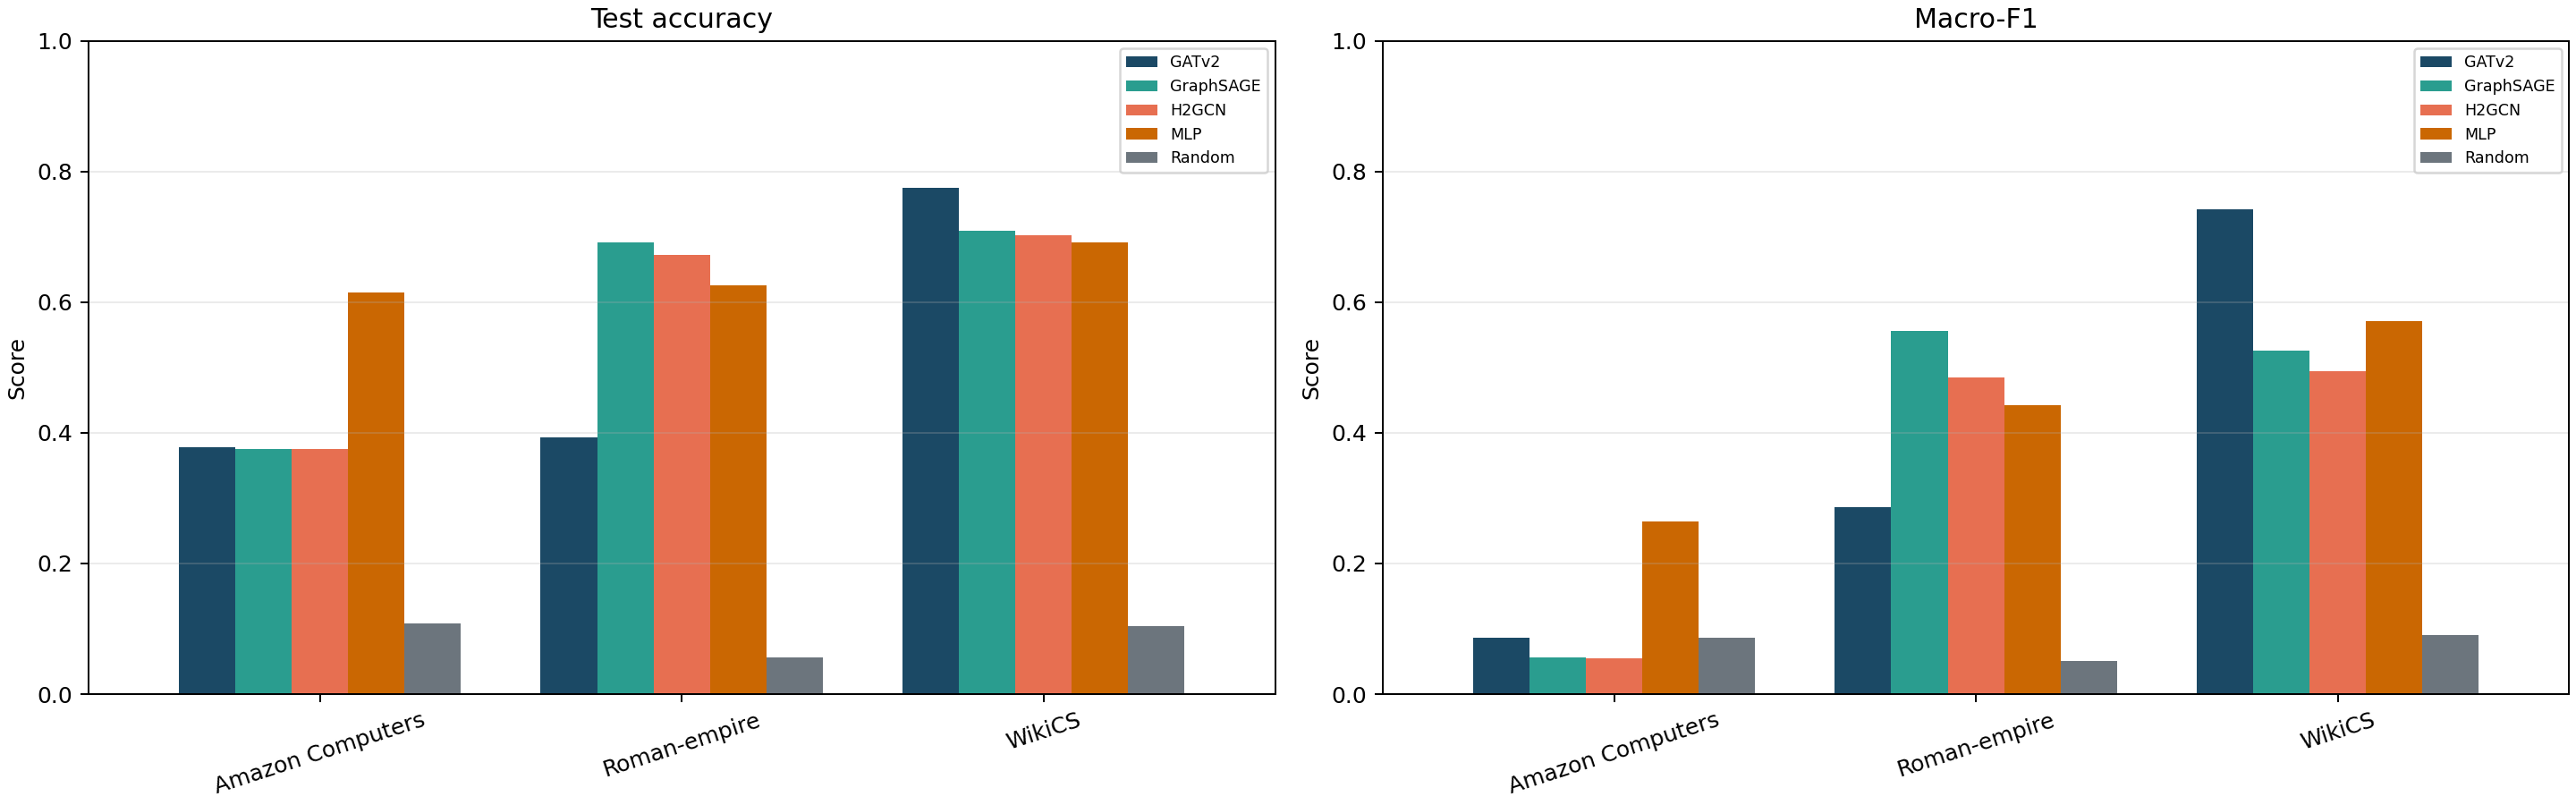
\includegraphics[width=0.95\linewidth]{results/plots/benchmark_comparison.png}
\caption{Accuracy and Macro-F1 across all model-dataset pairs.}
\end{figure}
\section{Roman-empire Analyses}
Roman-empire is the largest dataset by node count. We use two analyses across the GNN and MLP models (excluding Random): representation visualization and robustness. The visualization samples nodes only for plotting; training and evaluation use the complete graph. Robustness removes undirected edge pairs symmetrically and injects Gaussian feature noise, with repeated perturbation runs.
\begin{figure}[h]
\centering
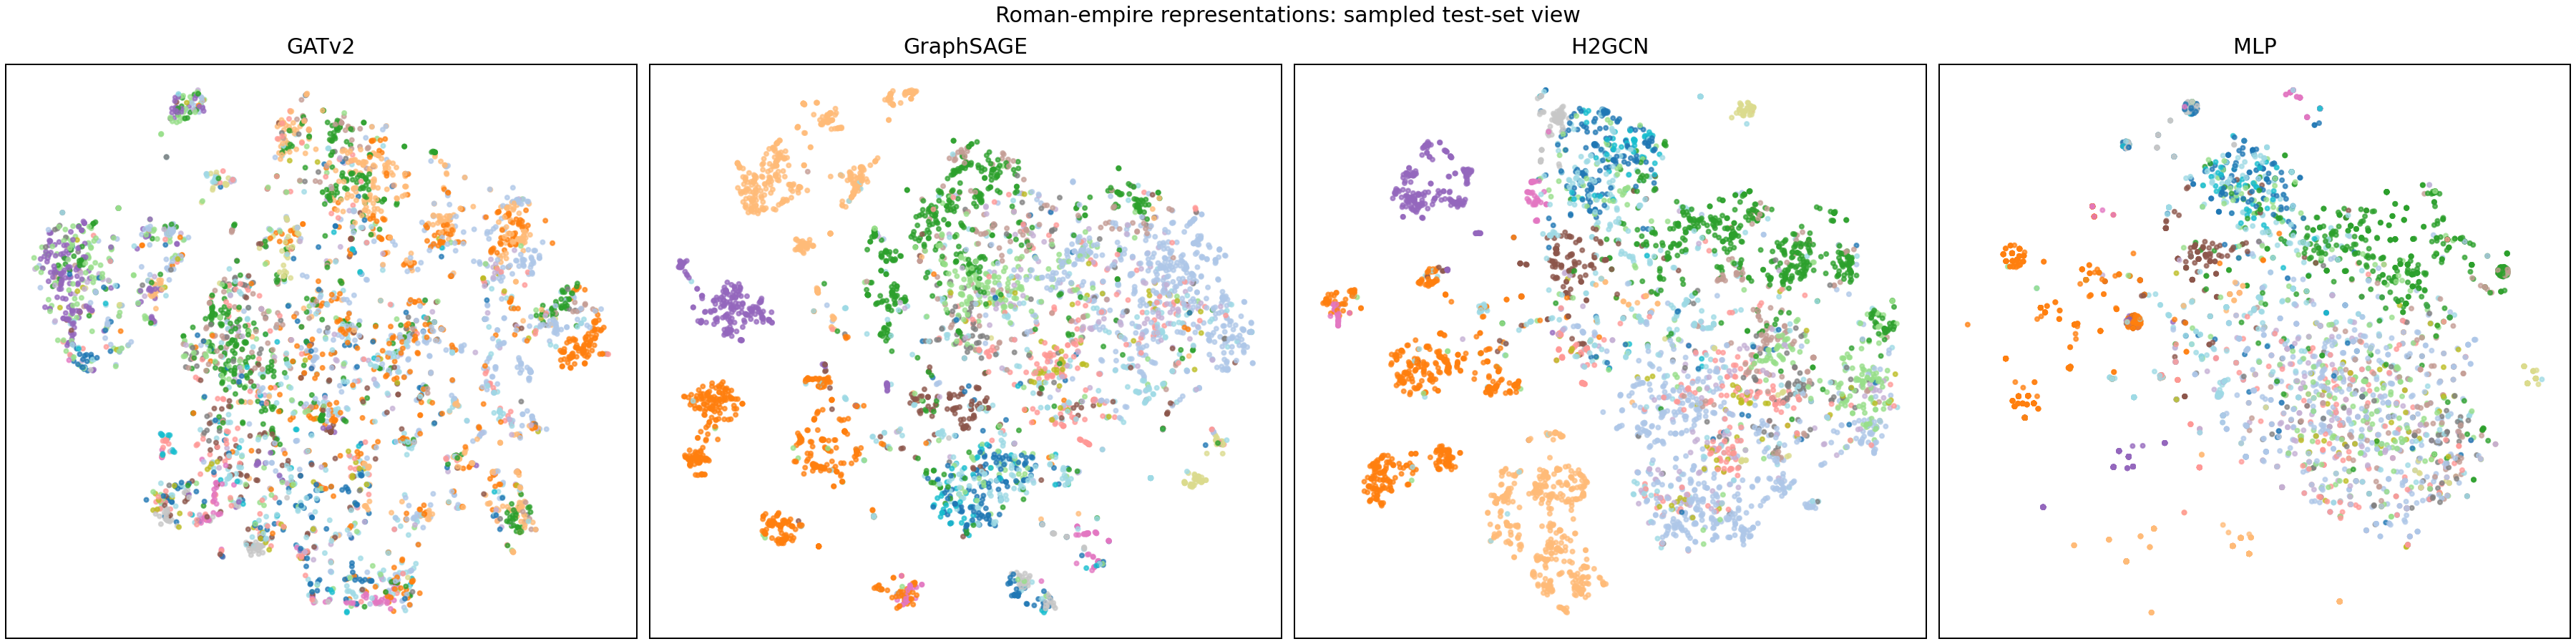
\includegraphics[width=0.95\linewidth]{results/plots/roman_embedding_tsne.png}
\caption{Sampled t-SNE view of penultimate representations on Roman-empire.}
\end{figure}
\begin{figure}[h]
\centering
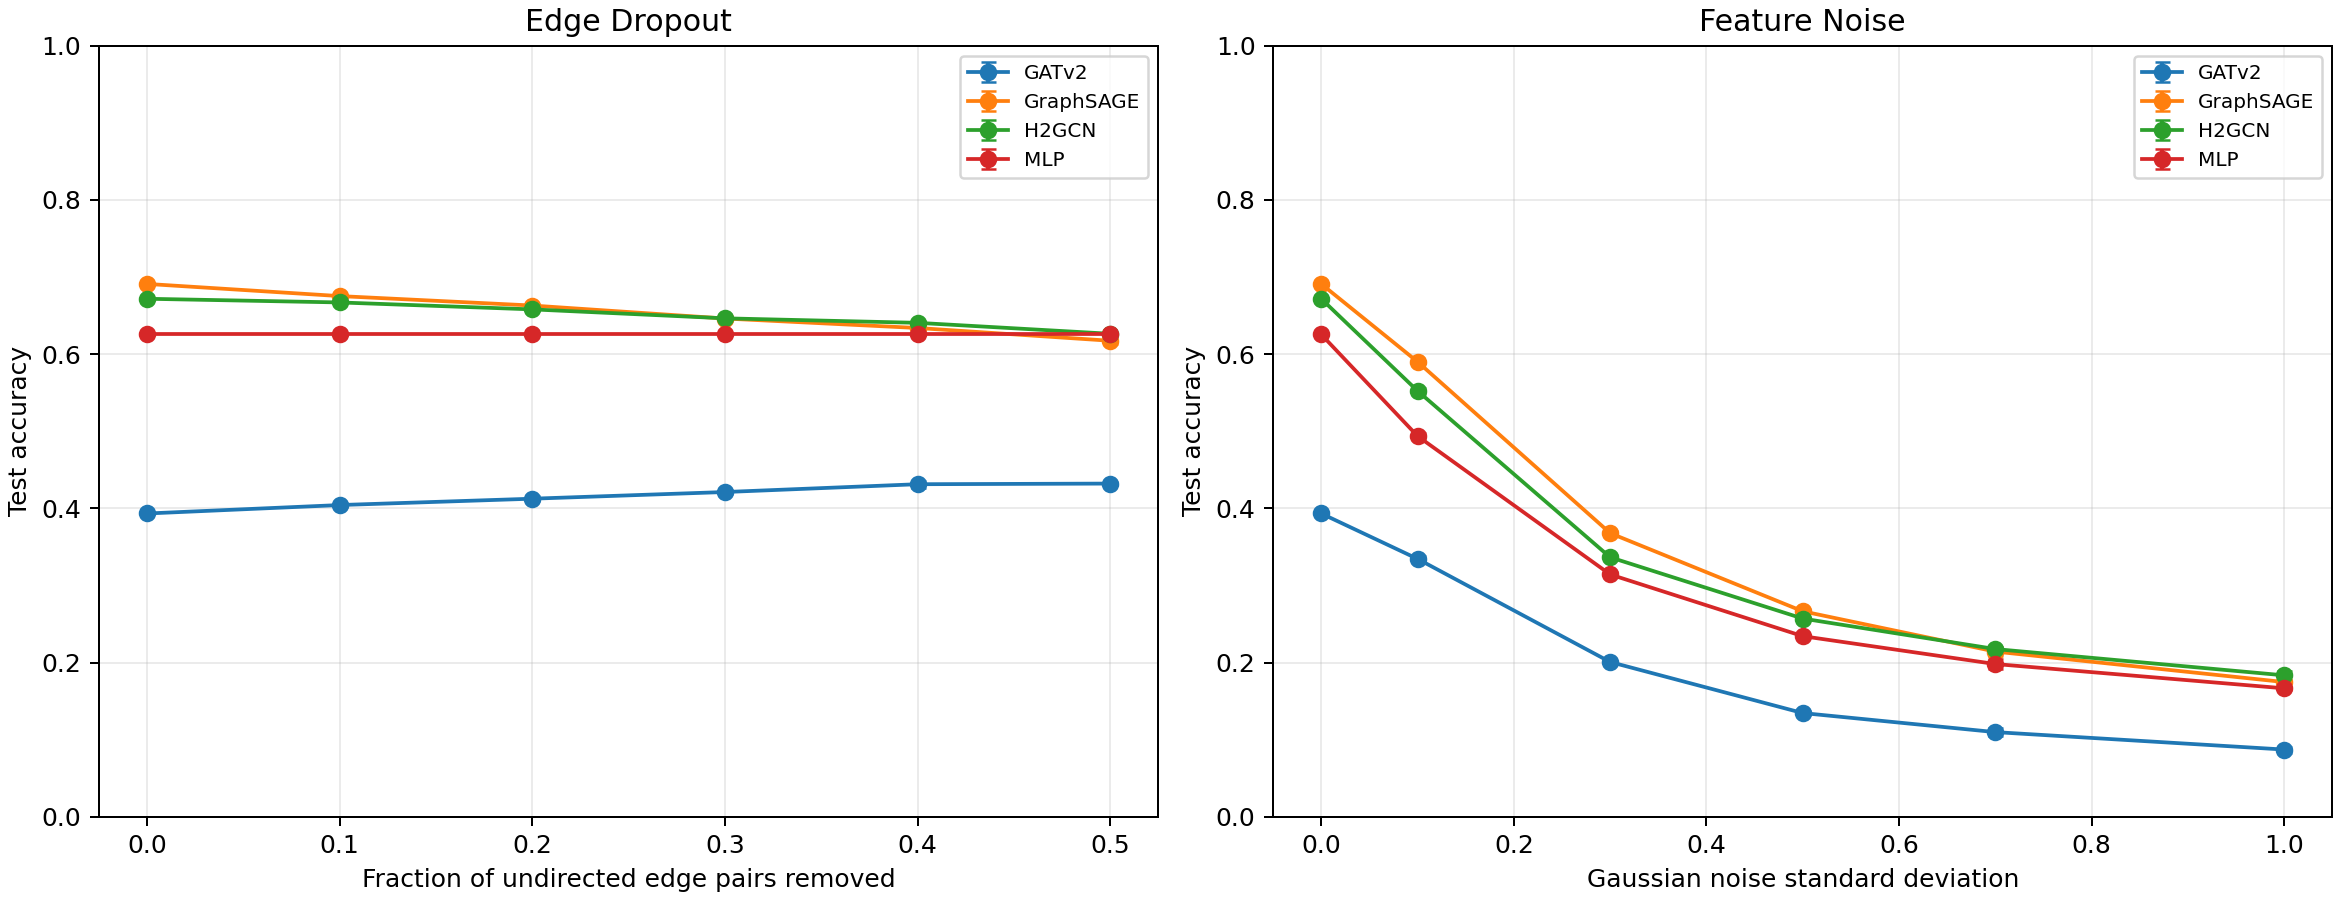
\includegraphics[width=0.95\linewidth]{results/plots/roman_robustness.png}
\caption{Robustness curves on Roman-empire.}
\end{figure}
\section{Limitations and Reproducibility}
The benchmark is transductive and uses full-batch message passing. t-SNE is qualitative rather than a metric of class separability. Results are hardware and software dependent, so the generated CSV files and checkpoint metadata should be treated as part of the result, not as optional supplements. Full runs use the configuration file; quick runs are explicitly marked in the experiment manifest.
\section{Conclusion}
The project is designed to test a structural hypothesis, not merely rank models. The final interpretation should emphasize whether performance changes with homophily, whether H2GCN's heterophily-aware design yields advantages on Roman-empire, and whether robustness failures arise from missing features, damaged topology, or the interaction of both.
\end{document}
